\documentclass{article}

\setlength\parindent{0pt}

\usepackage{../preamble/factory, ../preamble/font, ../preamble/math, ../preamble/math_font, ../preamble/style, ../preamble/theorem}

\newtheorem{thr}{Uppgift}

\begin{document}

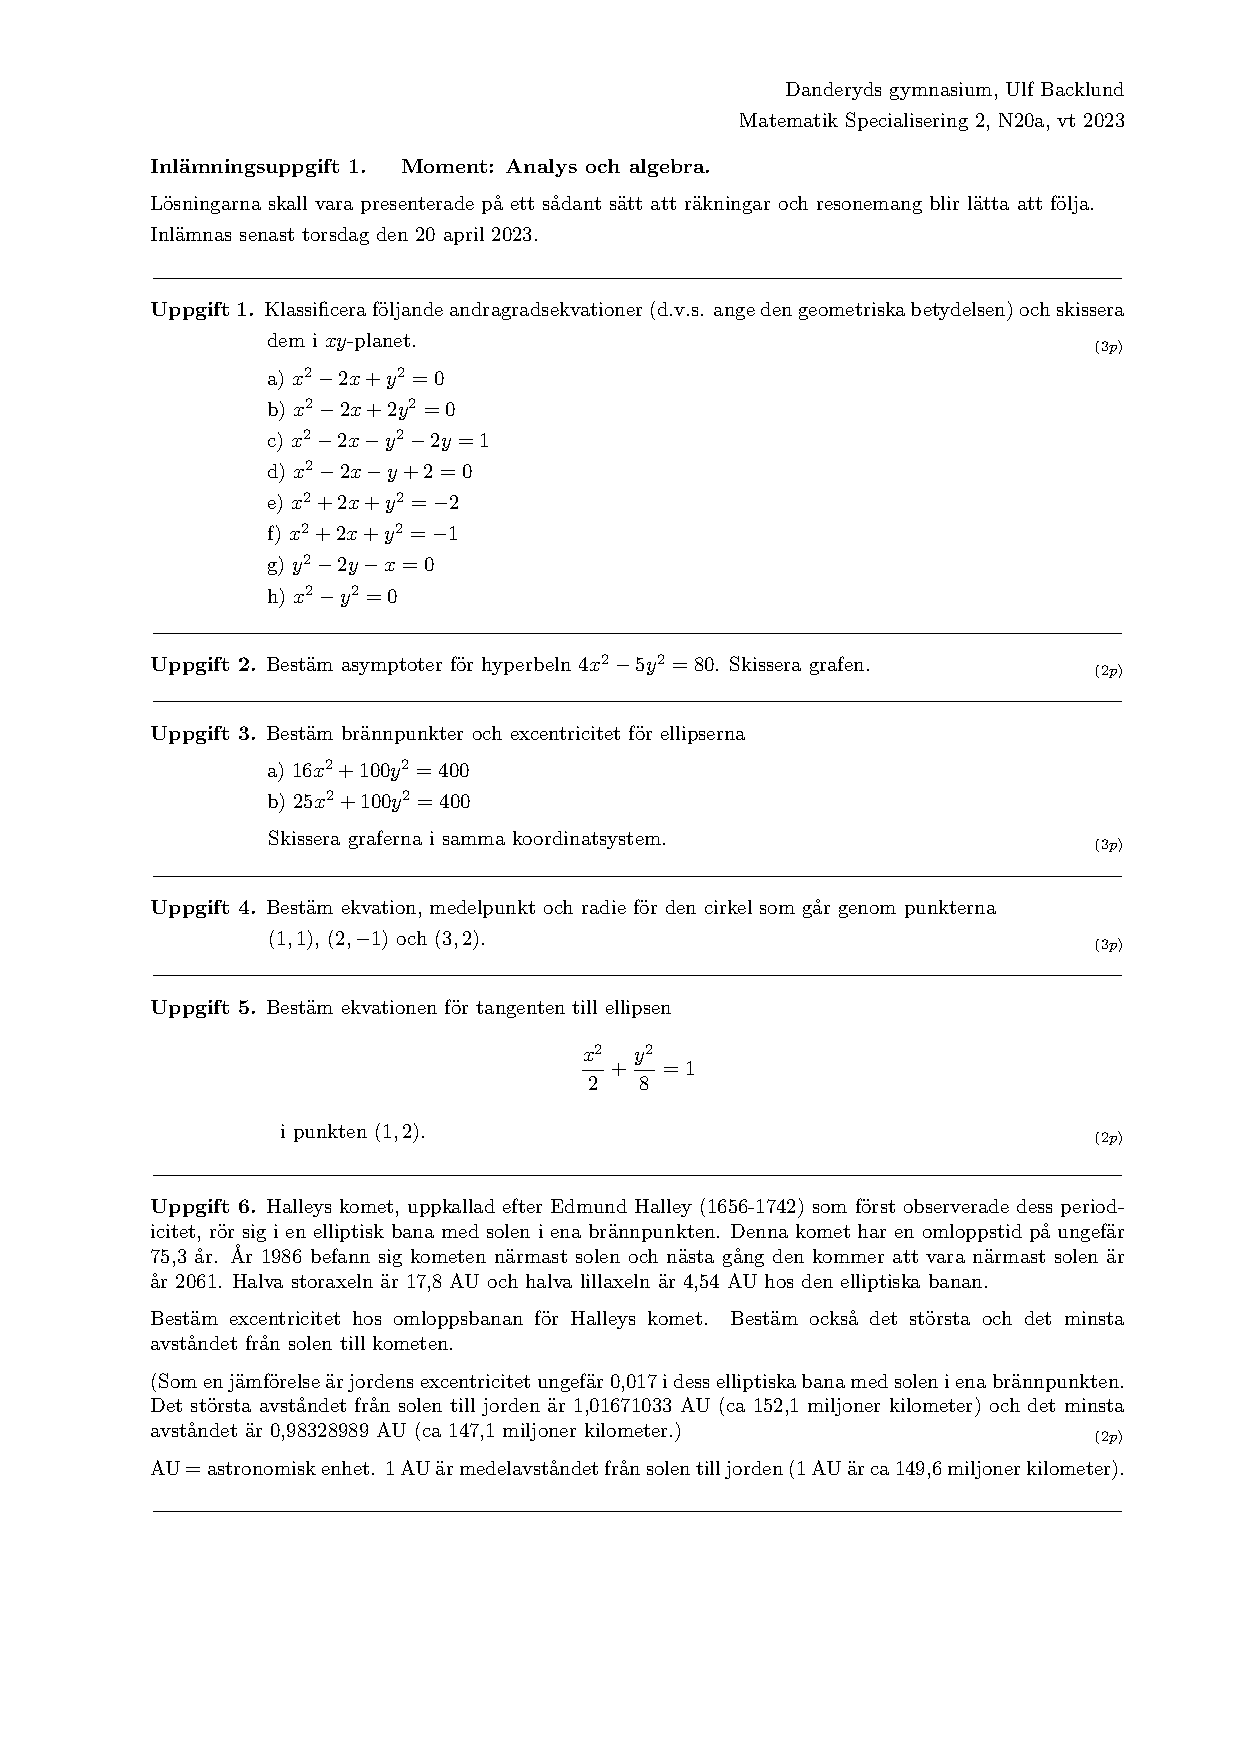
\includepdf{homework_1}

\newpage

\centerline{\large Matematik specialisering 2 inlämning 1}

\vskip 0.1cm

\centerline{\scriptsize Adam Amanbaev}

\vskip 1cm

% Uppgift 1 -------------------------------------------------------------------------------------------------------

\begin{thr}
Klassificera följande andragradsekvationer (d.v.s. ange den geometriska betydelsen) och skissera dem i xy-planet.
\end{thr}

\begin{enumerate}
    \item[a)] Genom att kvadratkomplettera $x$ i den givna ekvationen $x^2-2x+y^2=0$ får vi uttrycket $(x-1)^2+y^2=1$ vilket beskriver en cirkel med radien $r=1$ och medelpunkten $O=(1, 0)$ ty cirkelns ekvation är $(x-a)^2+(y-b)^2=r^2$ där radien är $r$ och medelpunkten är $O=(a, b)$. Cirkeln vi får ur ekvationen består av alla punkter med avståndet av radien $r=1$ från medelpunkten $O=(1, 0)$ vilket visas i Figure 1 nedan.
\end{enumerate}

\begin{figure}[h]
    \center
    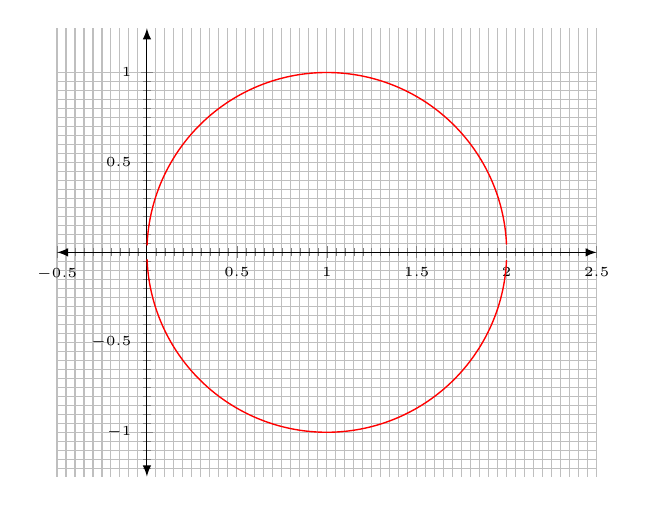
\begin{tikzpicture}
        \begin{axis}[
            xmin=-0.5, xmax=2.5,
            grid=both,
            axis lines=middle,
            minor tick num=9,
            axis line style={latex-latex},
            ticklabel style={font=\tiny},
            axis equal
            ]
            \addplot[line width=0.5pt, red, samples=5000]{-sqrt(2*x-x^2)};
            \addplot[line width=0.5pt, red, samples=5000]{sqrt(2*x-x^2)};
        \end{axis}
    \end{tikzpicture}
    \caption{\footnotesize Cirkeln som bildas av $x^2-2x+y^2=0$}
\end{figure}

\begin{enumerate}
    \item[b)] Genom att kvadratkomplettera $x$ i den givna ekvationen $x^2-2x+2y^2=0$ får vi uttrycket $(x-1)^2+2y^2=1$ som även kan skrivas som $\frac{(x-1)^2}{1^2}+\frac{y^2}{(\frac{1}{\sqrt{2}})^2}=1$ vilket beskriver en ellips som har medelpunkten $O=(1, 0)$ och brännpunkter på $(1 \pm \sqrt{1^2-(\frac{1}{\sqrt{2}})^2}, 0)$ vilket blir $(1 \pm \frac{1}{\sqrt{2}}, 0)$. Ellipsen visas i Figure 2 nedan.
\end{enumerate}

\newpage

\begin{figure}[h]
    \center
    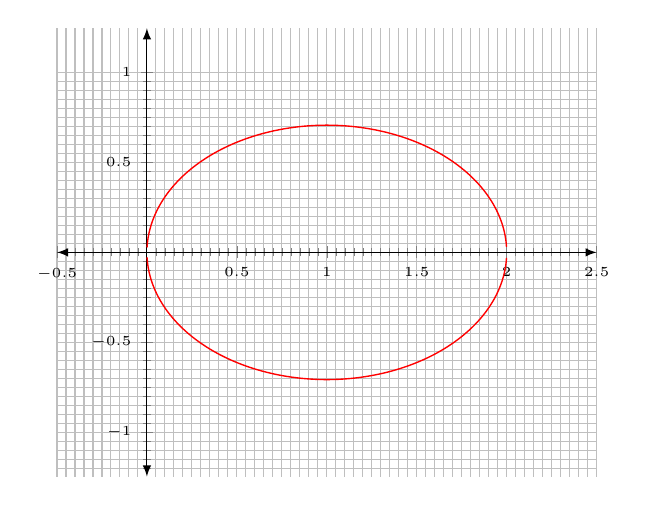
\begin{tikzpicture}
        \begin{axis}[
            xmin=-0.5, xmax=2.5,
            grid=both,
            axis lines=middle,
            minor tick num=9,
            axis line style={latex-latex},
            ticklabel style={font=\tiny},
            axis equal
            ]
            \addplot[line width=0.5pt, red, samples=5000]{-sqrt(x-0.5*x^2)};
            \addplot[line width=0.5pt, red, samples=5000]{sqrt(x-0.5*x^2)};
        \end{axis}
    \end{tikzpicture}
    \caption{\footnotesize Ellipsen som bildas av $x^2-2x+2y^2=0$}
\end{figure}

\begin{enumerate}
    \item[c)] Genom att kvadratkomplettera $x$ och $y$ i den givna ekvationen $x^2-2x-y^2-2y=1$ får man uttrycket $(x-1)^2-(y+1)^2=1$ vilket kan skrivas som $\frac{(x-1)^2}{1}-\frac{(y+1)^2}{1}=1$ vilket beskriver en hyperbel med medelpunkten $O=(1, -1)$ och brännpunkterna $(1 \pm \sqrt{1+1}, -1)$ vilket också är $(1 \pm \sqrt{2}, -1)$. Hyperbeln visas i Figure 3 nedan av de tunnare röda linjerna. De tjockare linjerna är hyperbelns asymptoter.
\end{enumerate}

\begin{figure}[h]
    \center
    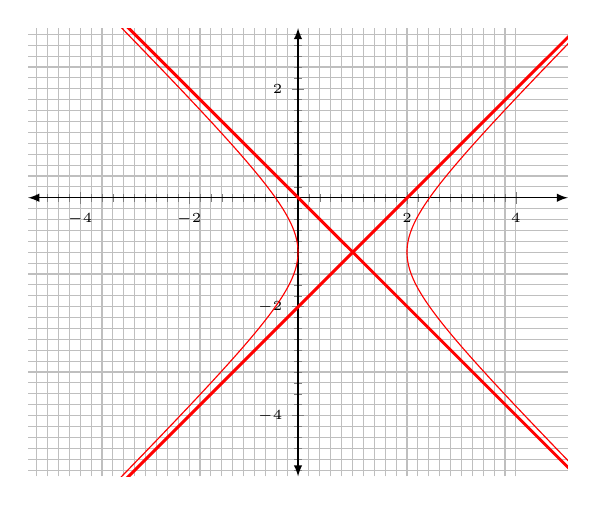
\begin{tikzpicture}
        \begin{axis}[
            xmin=-3.5, xmax=3.5,
            grid=both,
            axis lines=middle,
            minor tick num=9,
            axis line style={latex-latex},
            ticklabel style={font=\tiny},
            axis equal
            ]
            \addplot[variable=\t,samples=1000, red, domain=-35:35] ({1+sqrt(1)*sec(deg(\t))},{-1+sqrt(1)*tan(deg(\t))});
        \end{axis}
    \end{tikzpicture}
    \caption{\footnotesize Hyperbeln som bildas av $x^2-2x-y^2-2y=1$}
\end{figure}

\begin{enumerate}
\item[d)] Genom att komplettera $x$ i den givna ekvationen $x^2-2x-y+2=0$ får man uttrycket $(x-1)^2=4\frac{1}{4}(y-1)$ vilket beskriver en parabel med brännpunkten $(1, \frac{1}{4}+1)=(1, \frac{5}{4})$ och extrempunkten $(1, 1)$. Parabeln visas i Figure 4 nedan.
\end{enumerate}

\newpage

\begin{figure}[h]
    \center
    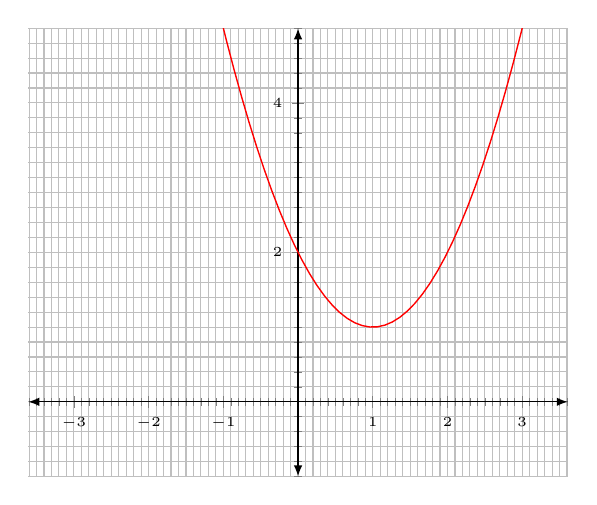
\begin{tikzpicture}
        \begin{axis}[
            xmin=-2, xmax=2,
            ymin=-1, ymax=5,
            grid=both,
            axis lines=middle,
            minor tick num=9,
            axis line style={latex-latex},
            ticklabel style={font=\tiny},
            axis equal
            ]
            \addplot[line width=0.5pt, red, samples=100]{x^2-2*x+2};
        \end{axis}
    \end{tikzpicture}
    \caption{\footnotesize Parabeln som bildas av $x^2-2x-y+2=0$}
\end{figure}

\begin{enumerate}
    \item[e)] Genom att kvadrattkompletera $x$ i den givna ekvationen $x^2+2x+y^2=-2$ får man uttrycket $(x+1)^2+y^2=-1$ vilket inte kan stämma ty summan av två kvadrater inte kan bli negativ. Ekvationen har därmed ingen geometrisk betydelse.
\end{enumerate}

\begin{enumerate}
    \item[f)] Genom att kvadrattkompletera $x$ i den givna ekvationen $x^2+2x+y^2=-1$ får man uttrycket $(x+1)^2+y^2=0$ vilket endast gäller då $(x+1)^2=0 \Och y^2=0$ vilket ger punkten $(-1, 0)$. Ekvationen beskriver alltså punkten $(-1, 0)$.
\end{enumerate}

\begin{enumerate}
    \item[g)] Genom att kvadrattkompletera $y$ i den givna ekvationen $y^2-2y-x=0$ får man uttrycket $(y-1)^2=4\frac{1}{4}(x+1)$ vilket beskriver en parabel med brännpunkten $(-1+\frac{1}{4}, 1)$ \\ $=(-\frac{3}{4}, 1)$ och extrempunkten $(-1, 1)$. Parabeln visas i Figure 5 nedan.
\end{enumerate}

\begin{figure}[h]
    \center
    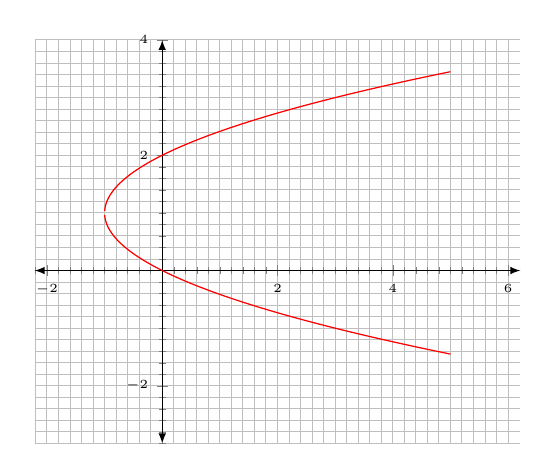
\begin{tikzpicture}[scale=0.9]
        \begin{axis}[
            xmin=-2, xmax=6,
            ymin=-3, ymax=4,
            grid=both,
            axis lines=middle,
            minor tick num=9,
            axis line style={latex-latex},
            ticklabel style={font=\tiny},
            axis equal
            ]
            \addplot[line width=0.5pt, red, samples=3000]{sqrt(x+1)+1};
            \addplot[line width=0.5pt, red, samples=3000]{-sqrt(x+1)+1};
        \end{axis}
    \end{tikzpicture}
    \caption{\footnotesize Parabeln som bildas av $y^2-2y-x=0$}
\end{figure}

\newpage

\begin{enumerate}
    \item[h)] Konjugatregeln i den givna ekvationen $x^2-y^2=0$ ger uttrycket $(x-y)(x+y)=0$ vilket gäller då $(x-y)=0 \Eller (x+y)=0$ vilket ger de två linjerna $y=x$ och $y=-x$. Linjerna visas nedan i Figure 6.
\end{enumerate}

\begin{figure}[h]
    \center
    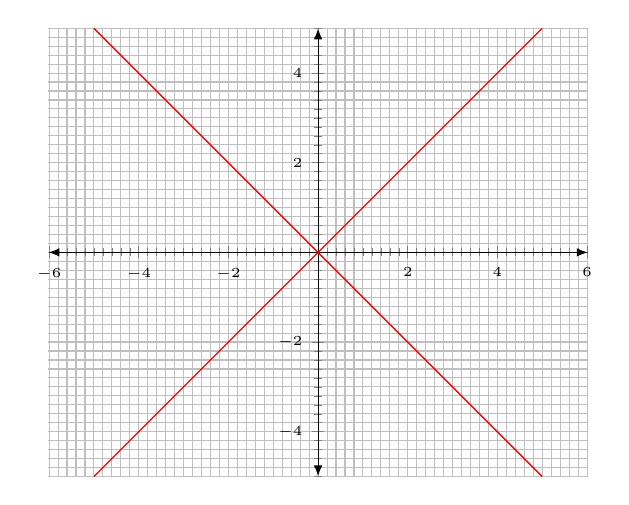
\begin{tikzpicture}
        \begin{axis}[
            xmin=-5, xmax=5,
            ymin=-5, ymax=5,
            grid=both,
            axis lines=middle,
            minor tick num=9,
            axis line style={latex-latex},
            ticklabel style={font=\tiny},
            axis equal
            ]
            \addplot[line width=0.5pt, red, samples=100]{x};
            \addplot[line width=0.5pt, red, samples=100]{-x};
        \end{axis}
    \end{tikzpicture}
    \caption{\footnotesize Linjerna som bildas av $y^2-x^2=0$}
\end{figure}

% Uppgift 2 ----------------------------------------------------------------------------------------------

\begin{thr}
Bestäm asymptoter för hyperbeln $4x^2-5y^2=80$. Skissera grafen.
\end{thr}

Genom att dela ekvationen med 80 får man uttrycket $\frac{x^2}{20}-\frac{y^2}{16}=1$. Asymptoterna beskrivs då av $(\frac{x}{\sqrt{20}}) \pm (\frac{y}{\sqrt{16}})=0$ vilket gäller då $y=4\frac{x}{\sqrt{20}} \Eller y=-4\frac{x}{\sqrt{20}}$. Asymptoterna är alltså $y=\pm 4\frac{x}{\sqrt{20}}$ och visas av de tjockare linjerna i Figure 7 nedan. Hyperbeln visas av de tunnare linjerna.

\begin{figure}[h]
    \center
    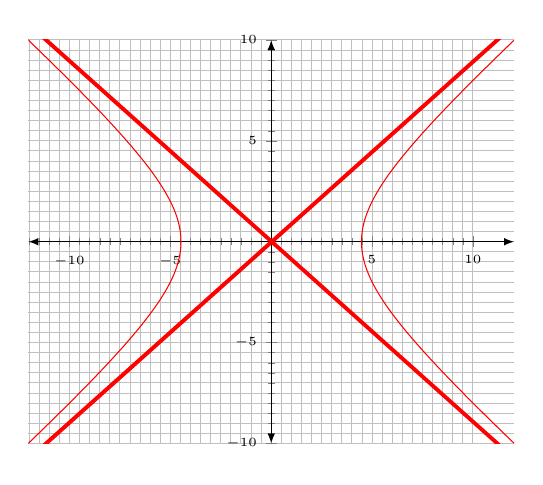
\begin{tikzpicture}[scale=0.9]
        \begin{axis}[
            xmin=-10, xmax=10,
            ymin=-10, ymax=10,
            grid=both,
            axis lines=middle,
            minor tick num=9,
            axis line style={latex-latex},
            ticklabel style={font=\tiny},
            axis equal
            ]
            \addplot[variable=\t, red, samples=1000, domain=-35:35]({sqrt(20)*sec(deg(\t))},{4*tan(deg(\t))});
        \end{axis}
    \end{tikzpicture}
    \caption{\footnotesize Hyperbeln som bildas av $4x^2-5y^2=80$ och dess asymptoter}
\end{figure}

% Uppgift 3 ------------------------------------------------------------------------------------------------

\newpage

\begin{thr}
Bestäm brännpunkter och excentricitet för ellipserna. Skissera graferna i samma koordinatsystem.
\end{thr}

\begin{enumerate}
\item[a)] $16x^2+100y^2=400 \Ekv \frac{x^2}{25}+\frac{y^2}{4}=1 \Ekv \frac{x^2}{5^2}+\frac{y^2}{2^2}$. Brännpunkterna blir $(\pm \sqrt{5^2-2^2}, 0)$ vilket även är $(\pm \sqrt{21}, 0)$. Excentriciteten, $\epsilon=\frac{\sqrt{a^2-b^2}}{a}$, blir $\epsilon=\frac{\sqrt{5^2-2^2}}{5}=\frac{\sqrt{21}}{5} \approx 0.92$. Ellipsen visas i rött i Figure 8 nedan.
\item[b)] $25x^2+100y^2=400 \Ekv \frac{x^2}{16}+\frac{y^2}{4}=1 \Ekv \frac{x^2}{4^2}+\frac{y^2}{2^2}$. Brännpunkterna blir $(\pm \sqrt{4^2-2^2}, 0)$ vilket även är $(\pm \sqrt{12}, 0)$. Excentriciteten, $\epsilon=\frac{\sqrt{a^2-b^2}}{a}$, blir $\epsilon=\frac{\sqrt{4^2-2^2}}{4}=\frac{\sqrt{12}}{4}=0.87$. Ellipsen visas i blått i Figure 8 nedan.
\end{enumerate}

\vskip 1cm

\begin{figure}[h]
    \center
    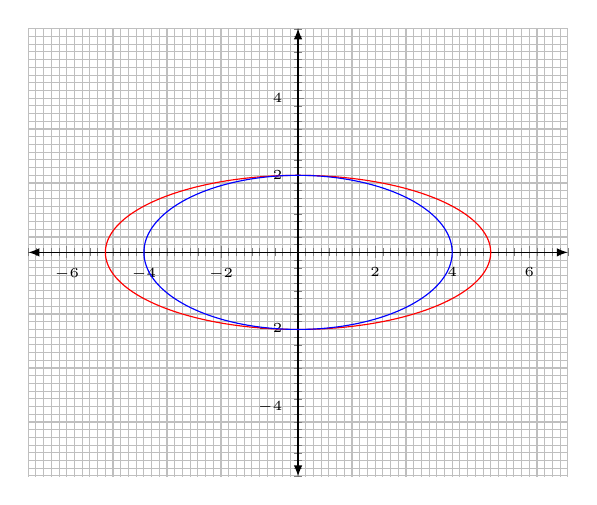
\begin{tikzpicture}
        \begin{axis}[
            xmin=-7, xmax=7,
            ymin=-4, ymax=4,
            grid=both,
            axis lines=middle,
            minor tick num=9,
            axis line style={latex-latex},
            ticklabel style={font=\tiny},
            axis equal
            ]
            \addplot[variable=\t, red, samples=1000, domain=-35:35]({5*sin(deg(\t))},{2*cos(deg(\t))});
            \addplot[variable=\t, blue, samples=1000, domain=-35:35]({4*sin(deg(\t))},{2*cos(deg(\t))});
        \end{axis}
    \end{tikzpicture}
    \caption{\footnotesize Ellipsen från (a) i rött och (b) i blått}
\end{figure}

% Uppgift 4 ----------------------------------------------------------------------------------------------

\newpage

\begin{thr}
Bestäm ekvation, medelpunkt och radie för den cirkel som går genom punkterna (1, 1), (2, -1) och (3, 2).
\end{thr}

Låt cirkelns medelpunkt vara $O=(x, y)$ och radien vara $R=r$. Eftersom medelpunkten är på samma avstånd från varje punkt på cirkeln gäller följande ekvationssystem enligt pythagoras sats: 

\begin{equation*}
    \begin{cases}
        (1-x)^2+(1-y)^2=r^2 \\
        (2-x)^2+(1+y)^2=r^2 \\
        (3-x)^2+(2-y)^2=r^2
    \end{cases}
\end{equation*}

\vskip 0.1cm

$\Ekv_{konjugatregeln}$

\vskip 0.1cm

\begin{equation*}
    \begin{cases}
        (-1)(3-2x)+(-2y)(2)=0 \\
        (2-x)^2+(1+y)^2=r^2 \\
        (3-x)^2+(2-y)^2=r^2
    \end{cases}
\end{equation*}

\vskip 0.1cm

$\Ekv_{konjugatregeln}$

\vskip 0.1cm

\begin{equation*}
    \begin{cases}
        2x-4y=3 \\
        (-1)(5-2x)+(2y-1)(3)=0 \\
        (3-x)^2+(2-y)^2=r^2
    \end{cases}
\end{equation*}

\vskip 0.1cm

$\Ekv$

\vskip 0.1cm

\begin{equation*}
    \begin{cases}
        2x-4y=3 \\
        2x+6y=8 \\
        (3-x)^2+(2-y)^2=r^2
    \end{cases}
\end{equation*}

\vskip 0.1cm

$\Ekv$

\vskip 0.1cm

\begin{equation*}
    \begin{cases}
        2x-4y=3 \\
        10y=5 \\
        (3-x)^2+(2-y)^2=r^2
    \end{cases}
\end{equation*}

\newpage

$\Ekv$

\vskip 0.1cm

\begin{equation*}
    \begin{cases}
        x=\frac{3+\frac{4}{2}}{2} \\
        y=\frac{1}{2} \\
        (3-x)^2+(2-y)^2=r^2
    \end{cases}
\end{equation*}

\vskip 0.1cm

$\Ekv$

\vskip 0.1cm

\begin{equation*}
    \begin{cases}
        x=\frac{5}{2} \\
        y=\frac{1}{2} \\
        r=\pm \sqrt{(3-\frac{5}{2})^2+(2-\frac{1}{2})^2}
    \end{cases}
\end{equation*}

\vskip 0.1cm

$\Ekv_{r \in \ZZ}$

\vskip 0.1cm

\begin{equation*}
    \begin{cases}
        x=\frac{5}{2} \\
        y=\frac{1}{2} \\
        r=\frac{\sqrt{10}}{2}
    \end{cases}
\end{equation*}

\vskip 0.1cm

$\Imp_{(x-x_{o})^2+(y-y_{o})^2=r^2}$

\vskip 0.6cm

Cirkelns ekvation blir $(x-\frac{5}{2})^2+(y-\frac{1}{2})^2=\frac{10}{4}$ där radien är $r=\frac{\sqrt{10}}{2}$ och medelpunkten är $O=(\frac{5}{2}, \frac{1}{2})$.

\newpage

% Uppgift 5 -------------------------------------------------------------------------------------------

\begin{thr}
Bestäm ekvationen för tangenten till ellipsen $\frac{x^2}{2}+\frac{y^2}{8}=1$ i punkten (1, 2).
\end{thr}

Ekvationen för en linje som tangerar en ellips $\frac{x^2}{a^2}+\frac{y^2}{b^2}=1$ är $y=mx+\sqrt{a^2m^2+b^2}$ där m är linjens lutning. En linje som tangerar den givna ellipsen har alltså ekvationen $y=mx+\sqrt{2m^2+8}$. Insättning av punkten $(1, 2)$ ger följande: 

\begin{equation*}
    2=m+\sqrt{2m^2+8}
\end{equation*}

$\Ekv_{m \leq 2}$

\begin{equation*}
    (2-m)^2=2m^2+8
\end{equation*}

$\Ekv$

\begin{equation*}
    m^2+4m+4=0
\end{equation*}

$\Ekv$

\begin{equation*}
    (m+2)^2=0
\end{equation*}

$\Ekv$

\begin{equation*}
    m=-2
\end{equation*}

$\Imp$

\vskip 0.5cm

Linjen som tangerar givna ellipsen i punkten $(1, 2)$ har ekvationen $y=-2x+\sqrt{2(-2)^2+8}$ vilket kan skrivas som $y=-2x+4$.

\newpage

% Uppgift 6 ----------------------------------------------------------------------------------------------

\begin{thr}
Halleys komet, uppkallad efter Edmund Halley (1656-1742) som först observerade dess period-icitet, rör sig i en elliptisk bana med solen i ena brännpunkten. Denna komet har en omloppstid på ungefär 75,3 år. År 1986 befann sig kometen närmast solen och nästa gång den kommer att vara närmast solen är år 2061. Halva storaxeln är 17,8 AU och halva lillaxeln är 4,54 AU hos den elliptiska banan. Bestäm excentricitet hos omloppsbanan för Halleys komet. Bestäm också det största och det minsta avståndet från solen till kometen.
\end{thr}

Vi vet att halva storaxeln är $a=17.8$ och halve lillaxeln är $b=4.54$. Låt oss använda skissen i Figure 9 nedan av en ellips och WLOG anta att solen ligger i högra brännpunkten:

\begin{figure}[h]
    \center
    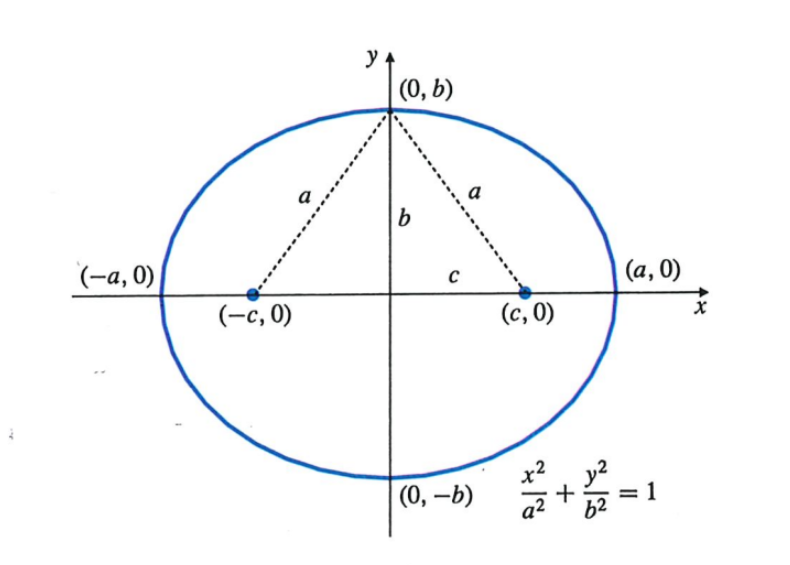
\includegraphics[scale=0.7]{./images/ellips}
    \caption{En ellips}
\end{figure}

Ellipsens ekvation blir $\frac{x^2}{(17.8)^2}+\frac{y^2}{(4.54)^2}=1$ där $c=\sqrt{a^2-b^2}=\sqrt{(17.8)^2-(4.54)^2} \approx 17.21$. Solen ligger då på brännpunkten $(c, 0)$. Excentriciteten hos den elliptiska banan blir $\epsilon=\frac{c}{a}=\frac{\sqrt{(17.8)^2-(4.54)^2}}{17.8} \approx 0.97$. Vi vet att $\epsilon QP = PF$ där $F$ är brännpunkten där solen är, $P$ är en punkt på ellipsen och $Q$ är där den vågräta linjen genom $P$ skär styrlinjen. Punkten $P$ som då minimerar avståndet $PF$ till solen blir den som minimerar avståndet $QP$. Den punkten blir $(a, 0)$ ty den är närmast styrlinjen. På samma vis blir $(-a, 0)$ punkten längst bort från solen då den är längst bort från styrlinjen. Minsta och största avståndet från solen till kometen blir alltså $(a-c)=(17.8-17.21)=0.59$ AU och $(c-(-a))=(17.21-(-17.8))=35.1$ AU respektive ty sträckorna ligger längs x-axeln.

\end{document}
